%------------------------------%
\selectlanguage{english}
\chapter{Abstraction-oriented resource awareness}
\label{chap:abstractions_and_resource_management}
\markboth{Abstraction-oriented resource awareness}{Chapter2}
%------------------------------%

\coolphrase {Where is the `any' key?}{Homer Simpson, in response to the message, ``Press any key''}

Defining and using software abstractions (such as classes, components and languages) are common operations when building applications.
Sometimes, it is useful to consider the problem of how instances of an abstraction consume computational resources.
For instance, computing the CPU consumed by all \textit{threads} running on a system is quite helpful for system administration purposes.
Another example is the necessity of knowing the number of instances of a given class when we are profiling applications.

As shown in the previous chapter, supporting resource management is a complex task that highly depends on the technology a system is running atop of.
In this chapter, we show that specific features of the software abstraction, which is being targeted, also influence the way resource management support is implemented.
%In this chapter we show that this support also depends on features of the software abstraction we are dealing with.
%In this chapter we show how the support that we can provide and its implementation are also driven by the specific features of the software abstraction.
Due to all these specific features there is considerable variability to consider when writing resource management tools; dealing with this variability is complex.

%This chapter mainly discusses how to ease the task of supporting resource-aware programming by taking into account the existence of many software abstractions.

This chapter mainly discusses how the usage of software abstractions poses new challenges when we are implementing support for resource consumption monitoring and reservation.
In particular, this chapter describes an abstraction -- components (Section \ref{sec:components-oriented-resource-awareness}), which is frequently used on top of MRTEs.
A comprehensive discussion on how this abstraction consumes resources is presented.
Moreover, state-of-the-art approaches, for handling features specific of components and other abstractions, are presented and their limitations discussed (Section \ref{sec:abstraction-specific-requirements}).
%We tackle (Section \ref{sec:component-leverage}) the issue of how to leverage component-based architectures - to reduce the overhead of dealing with resources - by specializing resource management techniques.
%Second, since new abstractions are constantly created nowadays, having generic and efficient mechanisms for controlling how they use resources may simplify the process of providing resource awareness support.
We then present the state of the art on simplifying the construction of tooling support for resource consumption accounting and reservation (Section \ref{sec:easy-tools-contruction}).

\section{Developer's View versus Tooling's View} \label{sec:chapter2-introduction}

Building abstractions is at the core of software development.
They are meant to tackle numerous problems in software engineering, ranging from providing better representation of the business logic to supporting applications' extensibility.
Interestingly, abstractions are not built from scratch; instead, they are implemented upon other abstractions provided by the runtime environment.
This leads to the well-known layered architecture where complex features are created using more simple concepts.
In the field of operating systems, processes are built relying on low-level concepts such as hardware interrupts, context-switch, and MMU hardware.
In the area of programming languages, recursive routines are implemented upon basic hardware stack manipulation.

Once a new abstraction is implemented and its invariants defined, you can use it without a complete understanding of the implementation details.
This has profound implications in the software development process; it now requires special tooling support because developers immediately start thinking in terms of such an abstraction.
For instance, showing plain assembler instructions while debugging applications is no longer good choice once you start coding your applications in a language that includes high-level concepts such as routines, loops, and conditional-statements.
In the same way, when a profiler is used to check the memory consumption of Java-based applications, the data produced is expected to reflect terms such as \textit{object} and \textit{class}.
Ideally, tools such as editors, debuggers, and profilers must be modified to make them aware of each new abstraction introduced in the development cycle.
Likewise, mechanisms to monitor resource consumption at runtime should also be modified.
Unfortunately, this is not always the case.
For instance, often developers lack the proper tools when they implement applications that execute in MRTEs.
A couple of illustrative examples are given below; the first is associated to the usage of \glspl{dsl}, the second is related to OSGi bundles.

\paragraph{The case of providing tools for new DSLs}
%When considering other abstractions, we can see that
Many of the newly designed DSLs are built on top of existing object-oriented languages runtime such as the JVM. 
Therefore, people in charge of optimizing, debugging and maintaining software applications can use the existing debuggers and profilers of these platforms. 
However, there is a clear mismatch between classical profilers used in object-oriented systems and the newly designed languages. 
Indeed, the concepts introduced in these new DSLs may not exhibit a straightforward mapping to the underlying object-oriented system.
As a consequence, it may be time consuming and complex to use a classical profiler to check applications that are based on these new languages.

For instance, active annotations allow developers to participate in the translation process of Xtend source code to Java code via library.
Such mechanism is often used directly by developers to introduce abstractions, and to define internal DSLs.
In the K3-AL\footnote{Available at \url{https://github.com/diverse-project/k3/wiki}} project, active annotations are used to create an open-class mechanism on top of Java \cite{Clifton:2000:MMO:353171.353181}. 
As a result, the annotation processor changes the program structure to implement this feature. 
It adds an indirection layer to invoke some methods (to $AASpect$), creates a new set of objects to represent part of the state of one conceptual object ($AASpectProperty$), and uses the Xtend extension method feature.
Figure~\ref{fig:k3-diagram} shows the result of this translation process. 
The code written by the developer is shown in Figure~\ref{fig:library-view}; to its right, Figure~\ref{fig:user-view} shows the user view (the code that can be written to use the open-class mechanism); and the runtime view is depicted in Figure~\ref{fig:tooling-view}.
In this example, an instance of an open-class is not represented by a single JVM object; instead, it is represented by many objects.  


\begin{figure}[ht]
\begin{subfigure}[b]{0.45\textwidth}
\centering
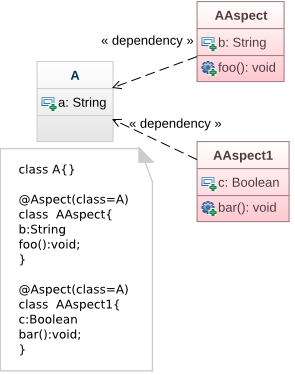
\includegraphics[width=0.75\linewidth]{chapter2/fig/library-developer-view.png}
\caption{Viewpoint of library developer}\label{fig:library-view}
\end{subfigure}
\hspace{0.3cm}
\begin{subfigure}[b]{0.45\textwidth}
\centering
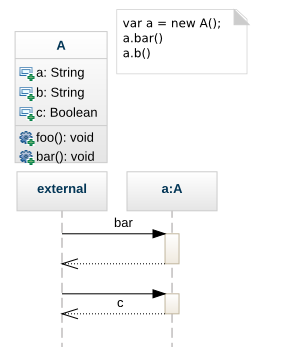
\includegraphics[width=0.75\linewidth]{chapter2/fig/user-view.png}
\caption{Viewpoint of library user}\label{fig:user-view}
\end{subfigure}
%\hspace{2.6cm}
\begin{subfigure} {\linewidth}
\centering
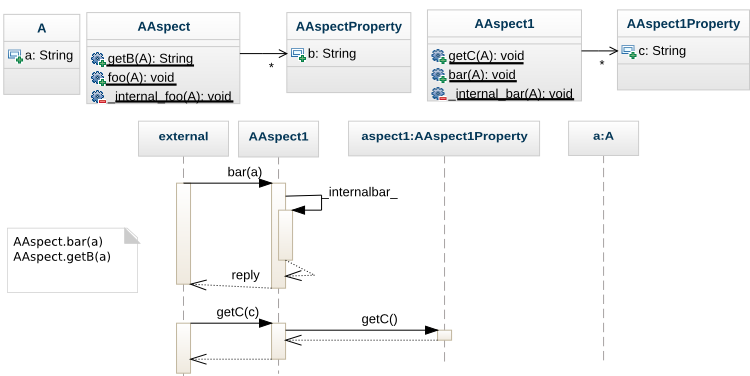
\includegraphics[width=0.9\linewidth]{chapter2/fig/tooling-view.png}
\caption{Tooling's view}\label{fig:tooling-view}
\end{subfigure}
\caption{Open-class mechanism in K3-AL, three views are shown: how the developer of the library see it (Fig \ref{fig:library-view}), how the user of the library see it (Fig~\ref{fig:user-view}), and how it is perceived by the tools (Fig~\ref{fig:tooling-view}).}
\label{fig:k3-diagram}
\end{figure}


\paragraph{The case of monitoring components}

\gls{CBSE} is an interesting example because it is widely used.
Curiously, although developers are encouraged to think in terms of high-level abstractions when software is written using components, little tooling support exists for resource awareness.
Indeed, in OSGi, a component framework, many bundles~\footnote{A bundle is a unit of deployment in OSGi.} are deployed on top of a single JVM instance.
Due to the communication mechanism used in OSGi, where objects are routinely shared, it is complex to decide which bundle should be accounted for the consumption of a particular object.
A possible approach is deciding that an object $O$ is being consumed by a bundle if $O$'s class was loaded using the classloader $C$ associated with such a bundle.
Then, we can use this mechanism to monitor per-bundle memory consumption. 
However, a profiler must perform considerable -- and costly -- amount of processing to collect such kind of data because it is not straightforwardly available in the JVM. 
%Since we know how to represent a bundle using Java concepts, this solution is feasible.
Given the widespread usage of OSGi, memory profilers often support collecting data regarding per-bundle memory usage.
Unfortunately, similar abstractions (components models), equally implemented atop of Java, are often not properly supported by such tools because they are not as popular as OSGi.
Hence, data must be manually aggregated when an application uses abstractions that are not supported by profilers; this is a considerable burden for developers.

The example of OSGi is also useful to highlight how some abstractions have specific requirements regarding resource consumption monitoring and reservation.
In the particular case of determining how many resources are being consumed by a bundle, it is noteworthy that there exist two ways of doing so when a bundle requests a service from another bundle.
Both approaches have pros and cons \cite{Miettinen2008,Maurel:2012:AME:2304736.2304763}.
In a first option, all resources used to satisfy a request are charged to the bundle that originally issued the request, no matter whether part of the computation is performed in other bundles.
In a second option, a bundle only consumes resources when it is executing its own code.
The important point is that, above the concern we present in the previous chapter regarding the mechanisms to support resource-aware programming, engineers also have to focus on features specific to each abstraction.

\paragraph{The problem at hand}
In this thesis, we argue that a \textit{mismatch}, between the developer's view and the tooling's view, exists when the concepts managed by the developers are not clearly reflected in the tools.
This mismatch may complicate the development of applications, as well as prevent the correctness of software systems.
We identify in this thesis, two ways in which such a mismatch may affect software development when new software abstractions are heavily used and, at the same time, support for resource-aware programming is also required:

%\todo{This two points are really close, bad}
\begin{itemize}
\item The creation of new software abstractions poses challenges for software developers because abstractions may have requirements that are not addressed by generic developing tools.
In particular, tools, such as profilers, and runtime monitors, may require modifications in order to reduce the gap between the user's view and the tools' view.
The problem is how to efficiently reuse the generic mechanisms of existing approaches to handle the specific requirements of new abstractions.

\item Since new software abstractions are constantly being defined, there is an increasing pressure to ease the creation of abstraction-specific tooling support.
Simplifying the definition of tools in order to support new abstractions is the issue in this case. 
\end{itemize}

In the rest of this chapter, we extensively discuss both concerns.

\section{Dealing with abstraction-specific requirements} \label{sec:abstraction-specific-requirements}
As claimed in the previous section, when a new abstraction is defined, there is a gap between the capabilities of existing tools and users' expectations.
Therefore, it is necessary to reduce this gap by modifying generic tools to make them capable of dealing with specific features of new abstractions.

In this section, we present the challenges that emerge when tooling support for resource management is being built.
To do so, we discuss the topic in two ways:

\begin{enumerate}
\item  We present how the mismatch between existing tools and users' expectation continuously emerges due to the increasing usage of DSLs to build applications.
This serves both to further motivate the research, and to present in details the technical complexity an engineer may face when new abstractions are used.
%In general, most problems we find, when programs are written using DSLs and resource awareness is required, can also be found in other contexts where different kind of abstractions are used.

\item We describe the specific features of a concrete kind of abstraction -- software components.
We do so because, despite of the fact that \gls{CBSE} is widely used in the industry, existing approaches to support resource awareness still have limitations.
\end{enumerate}

The presentation aims at highlighting the type of modifications that might be required in order to make an existing resource management tool capable of dealing with concepts defined in a new abstraction.
To guide the discussion, the following elements are given for both, programs written using DSLs and component-based systems:
\begin{itemize}
\item A \textbf{brief description} of the main elements of the abstraction, focusing on those features that impact resource management. 

\item Illustrative cases of \textbf{implementations} of these abstractions \textbf{on top of MRTEs}.
For instance, it briefly mentions components models that support Java.

\item An analysis of how \textbf{resources are consumed} by each type of abstraction.

\item \textbf{Special characteristics of these abstractions} to take into account when support for resource-aware programming is implemented.     

%\item \textit{Example of differences among concrete abstractions.}
%Since there are, for example, many DSLs, this point aims at analyzing differences among them.
%In this way, we show the high degree of variability that might complicate the development of resource-aware solutions.
%Instead of providing an exhaustive list of differences, we only show an illustrative one.

\end{itemize}

Afterwards, the \textit{state of the art} on providing support for resource awareness for new abstractions and, in particular, for component models is presented.
This is done in the form of a summarized discussion of existing approaches. 
The section ends by analyzing the limitations in these approaches. 


\subsection{DSLs: land of hungry abstractions} \label{sec:DSL-on-MRTEs}

%In Model-Driven Software Development (MDSD), models are abstractions of a software system and its environment~\cite{Stahl:2006:MSD:1196766, Fowler:2010:DSL:1809745}.
%A model contains a limited amount of information of a real system; thus, its utility is restricted to the domain it represents.
%The set of concepts and relationships that can be used in a concrete model are described in a Metamodel, which is also called Domain-Specific Language (DSL)~\cite{Fowler:2010:DSL:1809745}.
%In this way, a DSL describes a specific domain (e.g., state machines, interface definition language); while a model is then a concrete state machine in a real application, or a description of how components in a system interact.

In their seminal work~\cite{Czarnecki2000}, Czarnecki and Eisenecker embrace a broad notion of ``language'' that encompasses what are now known as internal and external \glspl{dsl} ~\cite{Fowler:2010:DSL:1809745}, but it also includes libraries of routines or classes that extend a programming language because they introduce new concepts and vocabulary.
A DSL describes a specific domain (e.g., state machines, interface definition language); thus, its utility is restricted to the domain it represents.
This widely used notion of ``language'' is what we have in mind when we discuss the problems associated to resource consumption in DSLs.
Figure~\ref{fig:dsl-hierarchy} shows a possible organization of these abstractions.

\begin{figure}
\centering
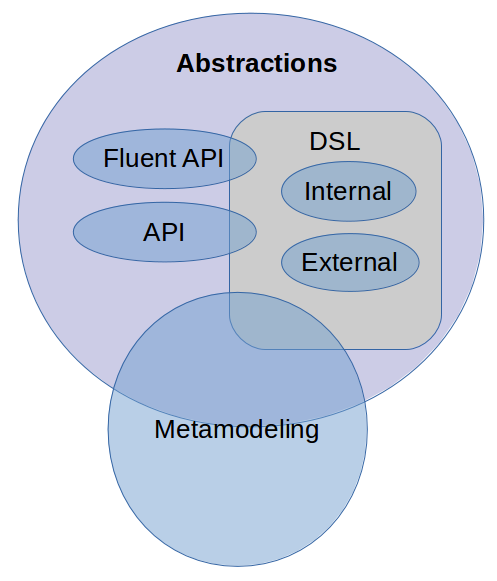
\includegraphics[scale=0.5]{./chapter2/fig/dsl-hierarchy.png}
\caption{Organizing abstractions as DSLs. This resembles the idea of ``language'' embraced by Czarnecki and Eisenecker~\cite{Czarnecki2000}.}\label{fig:dsl-hierarchy}
\end{figure}

The mechanisms used to represent concrete abstractions vary.
For instance, an internal DSL is embedded into a \gls{GPL}.
This is often done by relying on meta-programming facilities of a host language.
Likewise, design patterns and reflection are used to implement some forms of internal DSLs, such as fluent APIs, and annotation-based languages.
On the contrary, a ``\textit{program}'' written using an external DSL requires a separated translation process (i.e., compilation) in order to produce an artifact that can be integrated as part of an application.
It is then interesting that languages, regardless their representation, are always translated to concepts in a lower layer of the software stack.
Developers then find the gap between their view and the tooling's view. 
The problem is to find out how software abstractions consume computational resources.
%Both approaches have advantages and disadvantages that have been discussed elsewhere~\cite{Czarnecki2000, Stahl:2006:MSD:1196766}.
%One of the most important differences lays on the fact that external DSLs support the definition of arbitrary concrete syntaxes while internal DSLs don't.

%Internal DSLs can leverage all the features of their host languages, and it is easy to use constructors of the DSL as extensions of the host language.
%However, the concrete syntax of an internal DSL must be carefully crafted to cope with the constrains in the host language's syntax.
%On the contrary, there is complete freedom in deciding the concrete syntax of external DSLs; as a designer you can even choose not to use a textual syntax.
%Another interesting point is that Integrated Development Environment (IDE) support for internal DSLs is limited to the support provided to the host language.

%In a typical scenario, models are translated to source code written in some GPL to enable their subsequent compilation and execution.
%However, models are also useful in other tasks such as generating test cases \cite{Kiffe2009,Gutierrez2015}, simulating a system behavior \cite{Broenink2012,brosig2015a,Bocciarelli2015425}, and formally verifying software properties \cite{Holzmann2004,Henriksson2005101,Moffett2013,DiGuglielmo20132013}. 
%To write programs using a DSL (create models conforming to a metamodel), it is often necessary to use graphical~\cite{Kolovos:2009:RLA:1564600.1564699, Biermann:2006:GDI:2087202.2087244} or textual editors~\cite{Merkle:2010:TMT:1869542.1869564}.
%In general, the definition of a new ``language'' is a complex task because, depending on the language features, it may involve the definition of a complete infrastructure to deal with the DSL (i.e., editors, compilers, and simulators).
%Fortunately, approaches exist to ease the definition of DSLs.
%For instance, Xtext~\cite{Eysholdt:2010:XIY:1869542.1869625} is a well-known tool that is useful for defining new external DSLs (or for extending existing languages).
%It is an Eclipse-based framework which supports the definition of languages together with their syntaxes, semantic checkers, code generators and editors.

\paragraph{Support in MRTEs} 
As mentioned, concrete ``programs'' written in a DSL are typically translated to some host GPL.
This means that the DSL concepts are layered on top of concepts, such as \textit{classes}, \textit{objects}, and \textit{threads}.
Plenty of approaches exist for writing DSL-based applications that are transformed to be executed on top of MRTEs; in particular, many solutions target the Java language and the JVM.
For instance, the Xtext language workbench~\cite{Eysholdt:2010:XIY:1869542.1869625}, the Eclipse Modeling Framework~\cite{EMFModeling}, the meta-programming capabilities of languages such as Scala~\cite{Hofer:2010:MDL:1868294.1868307} and Clojure~\cite{Kelker2013} where internal DSLs can be defined and executed, the combination of annotations and annotation processor~\cite{Huang2008}, and intentional programming frameworks such as Meta-Programming System (MPS)~\cite{JetBrainsMetaProgrammingSystem(MPS),Voelter2014}.
Likewise, F\# applications, which execute in CLR, can use meta-programming support to write DSLs~\cite{Cheney:2013:PTL:2500365.2500586}; and the Boo language provides constructors that are easy to use for crafting DSLs~\cite{Rahien2010}. 

\paragraph{Abstractions and their resources consumption} 
Naturally, the resource consumption of a ``program'' written in a DSL depends on the DSL itself.
If a language is only used to describe data (without any executable semantics), then a program in such a language will consume memory.
On the contrary, if a language only describes behavior, a program written using such a language would use CPU to perform the computation.

An example is useful to illustrate how a DSL consumes resources.
Figure~\ref{lst:state-machine} shows a program written in a state machine language that resembles a DSL described in~\cite{Voelter2010}.
In this DSL, states, events and transitions are concepts defined by the DSL, but the guard conditions and the actions have a behavior that, as can be seen in the example, is plain imperative code.
To evaluate such sections of a state machine, CPU time is required.
In this case, it is necessary to know the translational semantic of the language in order to properly measure the CPU consumption.

\lstdefinestyle{statemachinelang}{
  belowcaptionskip=1\baselineskip,
  breaklines=true,
  frame=single,
  xleftmargin=\parindent,
  language=C,
  showstringspaces=false,
  basicstyle=\footnotesize,
  keywordstyle=\bfseries\footnotesize\color{green!40!black},
  commentstyle=\itshape\color{purple!40!black},
  identifierstyle=\footnotesize\color{black},
  stringstyle=\color{orange},
  otherkeywords={StateMachine, state, states, events, on, initial},
  tabsize=2,
}

\begin{lstlisting}[caption={State machine to control the door of a bus.},label={lst:state-machine},style=statemachinelang,frame=single]
StateMachine BusDoorManager
	events open_door() stop_requested() bus_stops() time_elapsed() 
	states (initial = DoorClosed) {
		state DoorClosed:
			on stop_requested() => ReachingStop
		state BusStopped:
			on open_door() => DoorOpen { light.on; door.open; timer.wait }
		state ReachingStop:
			on open_door() => OpeningDoor {}
			on bus_stops() => BusStopped {}
		state OpeningDoor:
			on bus_stops() => DoorOpen { light.on; door.open; timer.wait }
		state DoorOpen:
			on open_door_requested() => DoorOpen {}
			on time_elapsed() => DoorClosed { door.close; light.off }
	}
\end{lstlisting}

In other cases, the translation process of a DSL may only generate a structure for each ``program'', without any associated behavior.
Hence, only memory is consumed by the execution environment to represent a concrete model at run time.
For example, suppose we define a language to represent plants using the L-System formalism~\cite{Prusinkiewicz1990}.
A plant created by Prusinkiewicz et al.~\cite{Prusinkiewicz1990} using L-Systems, is depicted in Figure~\ref{lst:OL-system-example}.
The structures generated by this language may be simple strings of symbols (see \ref{fig:l-system-generated}).
The memory consumed by a L-System depends on the number of iterations, the rules defined, and the concrete data structure used to store the symbols
(it can be a string of characters, a tree, a list, or an array).
The important point is that users of this language should see this kind of structures as black-boxes.
Hence, in this example, the \textit{object} used to store the plant must be seen as structure of type \textit{OL-System} instead of as a simple Java \textit{string}.  


\lstdefinestyle{OL-systems}{
  belowcaptionskip=1\baselineskip,
  breaklines=true,
  xleftmargin=\parindent,
  language=C,
  showstringspaces=false,
  basicstyle=\footnotesize,
  keywordstyle=\bfseries\footnotesize\color{green!40!black},
  commentstyle=\itshape\color{purple!40!black},
  identifierstyle=\footnotesize\color{black},
  stringstyle=\color{orange},
  otherkeywords={contants, variables, initial, rules, iterations, angle, degrees, plant},
  tabsize=2,
}

\begin{figure}[ht]
\begin{mdframed}
\begin{subfigure}{0.45\textwidth}
\begin{lstlisting}[style={OL-systems}]
plant P0
	contants: + - [ ]
	variables: X F
	initial: X
	rules:
		X -> F[+X]F[-X]+X
		F -> FF
	iterations: 7
	angle: 20 degrees
\end{lstlisting}
\caption{DSL Code}\label{fig:l-system-code}
\end{subfigure}
\hspace{0.6cm}
\begin{subfigure}{0.45\textwidth}
\centering
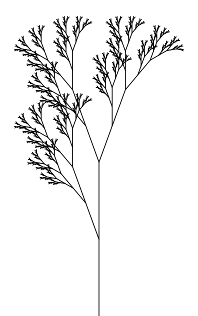
\includegraphics[scale=0.35]{./chapter2/fig/plant.png}
\caption{Graphical representation}\label{fig:plant}
\end{subfigure}
%\hspace{2.6cm}
\centering
\begin{subfigure} {0.8\linewidth}
\vspace{1cm}
\begin{lstlisting}[language=java, basicstyle=\footnotesize, stringstyle=\footnotesize\color{green!70!black}]
String P0 = "FF[+F[+X]F[-X]+X]FF[-F[+X]F[-X]+X]+F[+X]F[-X]+X";
\end{lstlisting}
\caption{Java code generated after translation (two iterations instead of seven)}\label{fig:l-system-generated}
\end{subfigure}
\end{mdframed}
\caption{Simple OL-System to generate a plant in two dimensions. On the left, the OL-System is represented using a DSL, on the right we show the tree that can be generated using such OL-System, below is the representation in Java.} \label{lst:OL-system-example}
\end{figure}

An important \textbf{feature to consider} by engineers who implement support \textbf{for resource awareness},
is that languages do not always provide well-defined boundaries.
For instance, an internal DSL may be transformed into a list of statements of the host language without defining a new routine or thread.
In a case like this, instrumentation is the only mechanism that can be used to achieve CPU consumption monitoring.
Interestingly, interaction between parts of an application written using DSLs can also impact the way resource accounting is done.
In the state machine example previously discussed, a state machine might trigger events in another state machine by simple executing some actions in one of its transitions.
In a situation like that, a resource accounting framework should properly determine the change of execution context; unfortunately, implementing this can be computationally expensive. 

%\extracomment{TODO}{
%One paragraph to highlight how the problem we find with programs implemented using DSLs also exist when other mechanisms are used to define abstractions.
%}

%The \textit{state machine} and \textit{L-system} languages clearly reflect differences between DSLs.
%These differences are not surprising.
%Languages consume resources in different ways; some languages only consume memory while others consume CPU or other resources.
%The capacity to monitor the consumption of a program written using a DSL is related to factors such as,
%the specific meaning of the involved concepts,
%and the translational semantic of the language.

%\extracomment{TODO}{Add discussion on how to ad plugins for Eclipse MAT and VisualVM}

%Profilers: visualvm
%
%low-Level profiling technologies: JVMTI, DTrace
%
%In~\cite{Xu:2013:PML:2491509.2491511} the authors propose a framework to detect memory leaks associated with Java containers.
%To do so, the framework explores the status of each container object with the goal of identifying leak patterns.
%
%LeakBots~\cite{Mitchell03leakbot:an} is an automated tool to detect memory leaks. It makes heavy
%use of information collected from the heap in order to identify the more likely structures leading to a leak.
%These tools collect data from the heap in order to automatically pinpoint a particular memory issue.
%The methods to collect the data are handwritten for efficiency reasons.
%Lots of data collected in these works is also available with our approach.


\subsection{On how software components consume resources} \label{sec:components-oriented-resource-awareness}

\glslink{CBSE}{CBSE} is a particularly interesting -- and concrete -- example of how tools that provide support for resource accounting and reservation must take into consideration features specific of each kind of abstraction.
In this section, we thoroughly discuss the concerns to address when dealing with component-based systems.  

\glslink{CBSE}{CBSE} aims at developing applications by reusing independent units of software \cite{cbse-conference, Crnkovic2011}.
Through the utilization of components, connectors and configurations, CBSE reduces the complexity in the development and maintenance of systems \cite{xadl,Medvidovic:2000,VanOmmering-et-al-00}.
%In addition to economical benefits such as reducing time to market and development cost \cite{SZYPERSKI2002}, there are also technical advantages in using CBSE. 
One of its technical advantages is that it facilitates the management of dynamic architectures
~\cite{DBLP:journals/ase/NittoGMPP08, Johnson:2015:CSM:2735960.2735979}
because it simplifies the implementation of features, such as, self-organizing the structure of a system, and self-adapting its behavior
\cite{PanzicaLaManna:2012:LDU:2304736.2304764, Johnson:2015:CSM:2735960.2735979,Zhang:2009:MVD:1509239.1509262}.
Likewise, many works~\cite{cbse-conference} have shown the benefits of using component-based approaches in open-world environments~\cite{baresi2006toward, Caporuscio:2010:AIA:1985522.1985547, Perez-Palacin:2010:PAO:1712605.1712614}.

In a general sense, the concept that embodies the idea behind software components can be defined as follows
\cite{Crnkovic2011}:

\begin{description}
\item[Definition 1:] A \textit{Software Component} is a software building block that conforms to a component model. 
\item[Definition 2:] A \textit{Component Model} defines standards for (i) properties that individual components must satisfy; and (ii) methods, and possibly mechanisms, for composing components.
\end{description}

Plenty of diversity exists in current component models and frameworks \cite{Heineman2001, SZYPERSKI2002, Crnkovic2011}.
They tend to target different technologies, aim at different use cases, provide support for different concerns, and use different design principles.
Crnkovic et al. \cite{Crnkovic2011} propose properties that can be used to classify component models; we are interested in those models that have the following properties:

\begin{description}
\item[Modeling capabilities:] it is common to provide a mechanism for modeling the system architecture during the development phase; this results useful to reason about the system.
In addition, it is possible to support some form of reflection for querying the architecture of a system at runtime.
Component models that include both features are the target of our research.

\item[Deployment of components at runtime:] since, we are dealing with the problem of supporting resource awareness in open environments, we focus on component models that allow component deployment at runtime.
Many component models are able to cope with the necessity of adaptation through, for example, the deployment of new modules, the instantiation of new services, and the creation of new bindings between components~\cite{Porter:2014:RMC:2602458.2602471, Zheng:2014:RCC:2679601.2680405, Irmert:2008:RAS:1370018.1370036, Ghezzi:2010:QDD:2163764.2163774}.
\end{description}

Other properties worth mentioning in this thesis are those that describe how components communicate.
For instance,  whether the concept of \textit{port} is implemented; if there exists distinction between \textit{required} and \textit{provided interfaces}; characteristics of the \textit{interface language}; and what is the \textit{communication type} (synchronous, unicast, and others).
Our interest in these properties is limited to understanding what mechanisms are used to support interaction between components, how are these mechanisms implemented, and how this interaction affects the way in which we deal with resource consumption monitoring and reservation.

\paragraph{Support for component-based engineering in MRTEs}
An important property of component models is its implementation support.
The discussion in this research is limited to those that have been implemented for MRTEs.
Several component models that provide support for MRTEs have been proposed in both the industry and the academy.
Among others, we can mention Enterprise Java Beans (EJB) \cite{OracleEJB3.0}, the Open Services Gateway Initiative (OSGi) \cite{OSGI:r5}, 
Fractal \cite{Bruneton:2006:FCM:1152333.1152345}, 
SOFA 2.0 (Software Appliances) \cite{Bures2006}, Palladio \cite{Becker:2010:PCM:1712605.1712651}, and Kevoree~\cite{morin09a,leger2010reliable}.
It is interesting how these component models have different properties when it comes to \textit{modeling capabilities}, \textit{architecture of the system supported}, and \textit{constructs for interaction among components}.
However, they also differ in how components are represented on top of MRTE concepts; in other words, they follow different approaches to implement the component framework itself.

\paragraph{How components consume resources}
Interestingly, components provide boundaries between different software entities, which are forced to communicate through well defined interfaces; it is then possible to write \gls{QoS} contracts associated to these interfaces \cite{Beugnard774917}.

It is important to remember the difference between component type and component instance when we discuss the resource usage of these systems.
Indeed, instances may have a state while component types are stateless.
The distinction is important because all instances of a single component type share the same implementation.
As a consequence, it is not simple to define how a component consumes resources.
For example, the memory consumed by an instance includes those \textit{objects} used for the component framework to represent the instance itself, its ports, and bindings; it also includes the state of the component. 
However, it cannot include the memory used to store the component's code since it is shared among many instances.
Monitoring CPU and network consumption is even harder, because the code responsible for the consumption is shared.
To solve this problem, a context is associated with each component in order to determine at runtime the instance responsible for the execution of a given operation that is using resources.
Interestingly, the exact representation of this context depends on the component model, and it may impact the performance of component-based systems.
A common way to define this context, is associating a set of threads to a component.

To summarize, the resources consumed by a component comprise (but are not limited to): its state, the time-shared resources it uses (CPU, network), the space required to store data and code shared among all instances of a component type, and the temporary space needed to execute the component.       

\paragraph{Contracts on resource consumption}
\glslink{QoS}{QoS} contracts serve, among others, to describe how components consume resources.
They simply express what resources will be consumed by a component to perform some action. 
In writing such contracts, it is better for developers to use platform-independent metrics.
Indeed, doing otherwise hinders the interpretation of a contract when components are deployed in different platforms.
For instance, if $n$ CPU cycles are required to handle a request, this $n$ may, in fact, represent different amount of CPU time depending on the architecture.
This is the reason why, the number of bytecode instructions to be executed, which is platform-independent, offers the following advantages:
\begin{itemize}
\item It is easy to control the admission of components because each platform knows how many bytecode instructions it is able to execute in an interval of time.
\item A portable framework for resource consumption monitoring is easier to implement.
\item Different measurements are easy to compare, even across platforms, because they use the same metric.
\end{itemize}
Besides the metrics used, the exact interpretation of a contract is also a fundamental concern.
Contracts may express properties for just one component and a single type of resources, but they can also express how should be the usage of resources in more complex scenarios where different components and types of resources are involved.

\paragraph{Specific features to consider}
A first issue to take into consideration is \textit{how to account for resource consumption in the presence of interaction between components}.
Usually, components are organized as clients and providers, where a component (provider) performs operations on behalf of other components (clients).
It is then possible to account for resource consumption in two ways \cite{Miettinen2008,Maurel:2012:AME:2304736.2304763}:

\begin{description}

\item[Indirect accounting:] all the resources consumed to serve a request that was originated in a component $A$ are accounted to $A$ (See Figure~\ref{fig:indirect-accounting}).
In other words, there is no resource consumption accounted to service providers.

\item[Direct accounting:] the resources consumed during
interaction are accounted to the provider (See Figure~\ref{fig:direct-accounting}).
For instance, the CPU used by a code that belongs
to component $A$ is accounted to $A$, no matter if the code is executed on behalf of a client.
\end{description}

Both ways have advantages and disadvantages.
In the case of direct accounting, if a provider is
called in an endless loop, the resource usage will be accounted
to the provider instead of to the client that executes such a loop.
On the contrary, if a service is poorly implemented, in indirect accounting the user of the service is identified as the responsible.

\begin{figure}[ht]
\begin{subfigure}{0.45\textwidth}
\centering
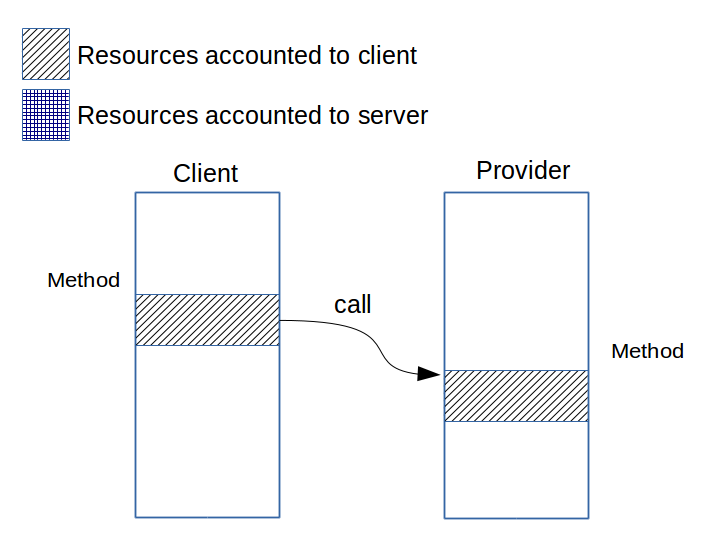
\includegraphics[scale=0.35]{./chapter2/fig/indirect-accounting.png}
\caption{Indirect Accounting}\label{fig:indirect-accounting}
\end{subfigure}
\hspace{0.6cm}
\begin{subfigure}{0.45\textwidth}
\centering
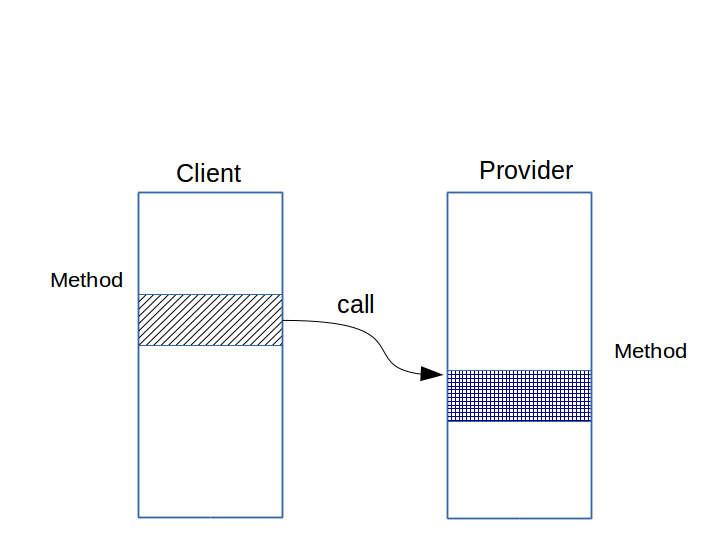
\includegraphics[scale=0.35]{./chapter2/fig/direct-accounting.png}
\caption{Direct Accounting}\label{fig:direct-accounting}
\end{subfigure}
\caption{The two mechanisms to account for resource consumption when components interact.} \label{fig:accounting-methods}
\end{figure}


Similarly, there is another problem to determine the memory consumption of components.
Often, objects are created by a component (allocator) and used in other components (clients).
This happens during interaction among components, when they exchange data in the form of objects (e.g., a service component creates new objects in response to clients' requests).
%Two criteria exist to account for memory consumption in component-based systems
For instance, a component may allocate space for an object, then send it to a client, and finally forget about it.
In that case, it is not clear what component should be accounted for the memory consumed by that particular object; it can be either the client or the original allocator.
Both approaches have pros and cons.
The intuition dictates that if a component is preventing an object of being collected it should be accounted for that particular block of memory.
However, such an approach may be dangerous if a buggy (or malicious) provider creates objects unnecessarily big, sends them to clients, and forgets about them; in that case, it would be hard to identify the provider as the source of excessive consumption. 
Most existing solutions for memory consumption follow a fixed criterion, either account always for the allocator or for the component preventing the object's collection.

A second aspect is to decide \textit{where should be implemented} the mechanism for resource consumption monitoring and reservation.
Essentially, this consists in, selecting which actors implement the mechanism and policies to manage resources, and deciding if the actors collaborate to achieve their goal \cite{Crnkovic2011}.
Indeed, many component models provide no facilities for managing \glspl{EFP}.
In these cases, the mechanism used to handle a property is left to the designers of each application.
This facilitates the creation of EFP management policies that are specifically tuned towards a system, and also allows the use of multiple policies in a system.
On the contrary, other approaches favor the separation of concerns between functional and non-functional aspects.
Hence, components are only allowed to address functional aspects, while containers are in charge of wrapping components to guarantee EFPs.

Finally, some differences among component models impact the implementation of mechanisms for resource consumption monitoring.
For instance. Kevoree and OSGi provide different methods for interaction between components.
In Kevoree, components communicate with each other through ports.
It is straightforward to identify in the code when a component is requesting a service because a single interface (port) is used to do so, no matter if a component is using different ports. 
As a consequence, an automated tool can easily instrument the code to detect when components are communicating.
On the contrary, OSGi uses plain Java interfaces and objects to connect bundles.
In that cases it is more complex to detect when components are communicating because a bundle can communicate with several services using different interfaces. 

%Franz Brosch, Heiko Koziolek, Barbora Buhnova, Ralf Reussner: Architecture-Based Reliability Prediction with the Palladio Component Model. IEEE Trans. Software Eng. 38(6): 1319-1339 (2012)
%
%Sam Malek, Marija Mikic-Rakic, Nenad Medvidovic: A Style-Aware Architectural Middleware for Resource-Constrained, Distributed Systems. IEEE Trans. Software Eng. 31(3): 256-272 (2005)
%
%Anne Koziolek, Ralf Reussner: Towards a generic quality optimisation framework for component-based system models. CBSE 2011: 103-108
%
%Marco Autili, Paolo Di Benedetto, Paola Inverardi: Context-Aware Adaptive Services: The PLASTIC Approach. FASE 2009: 124-139
%
%Mauro Caporuscio, Antinisca Di Marco, Paola Inverardi: Model-based system reconfiguration for dynamic performance management. Journal of Systems and Software 80(4): 455-473 (2007)
%
%Marco Autili, Paolo Di Benedetto and Paola Inverardi, Hybrid Approach for Resource-based Comparison of Adaptable Java Applications (2012), in: Journal of Science of Computer Programming (SCP)

\subsection{State of the art on dealing with abstraction-specific features}

This section presents a several approaches that tackle the problem of providing tooling support for developing applications using new software abstractions.
In particular, it discusses some solutions for debugging domain-oriented abstractions.
Furthermore, this section describes several mechanisms to monitor how components consume resources and to isolate such consumption.

\paragraph{Providing resource awareness support for DSLs}
Among the development tools that help to software maintenance, debuggers and profilers generally support mainstream concepts such as \textit{classes}, \textit{objects}, \textit{methods}, and \textit{call stack}.
Using them, it is possible to determine, at some extent, how applications are consuming resources.
However, we have found that limited support exists for extending the usage of these tools in order to make them understand more specific concepts (e.g., classes representing the business logic of an application, or a design pattern).
In other words, they are not fully capable of dealing with resources at per DSL level.
Yet, some related works do exist; they aim at reducing the gap between the developer's view and the tools' view.
In particular, the problem of offering debugging support for DSL constructs have been discussed.
In Xtext~\cite{Eysholdt:2010:XIY:1869542.1869625}, languages that produce code in the base language (i.e., Java) may profit from mostly automatic debugger support.
When the newly define DSL is transformed into the base language, the system keeps traces between the two models (source and destination).
Using these traces, a debugging infrastructure is able to identify what constructor is being executed in the original DSL.
Meanwhile, Voelter \cite{Voelter2010} discusses how to add debugging capabilities to a DSL when the MPS language workbench is used.
In this case, no trace model is required; instead, every concept of a language that requires debugging support must implement a set of interfaces to guide a generic debugging framework.
Similar works have been conducted \cite{vandenBrand:2005:TGD:1705513.1705667} for the ASF+SDF Meta-Environment \cite{vandenBrand20013}, defining a generic debugging framework that can be customized for DSLs.
Finally, mechanisms to build various tools for new languages are described in \cite{Henriques2005}.
Based on attribute grammars, and implemented using the LISA system \cite{Mernik2002}; the tools proposed include editors, inspectors, debuggers and visualizers.

\paragraph{Component-based systems}

Many works address the issue of supporting resource consumption monitoring in component-based systems.
In addition, some existing approaches present solutions for the isolation of resource consumption among components running on top of a single MRTE instance.
Unfortunately, most approaches are limited to a specific component model; in particular, works exist to solve the problem for both EJB and OSGi.

\textit{EJBMemProf}, a framework for profiling the memory consumption in EJB is presented in \cite{Meyerhoefer2005}.
The main idea of this framework is instrumenting applications' code to trigger an event each time an object is allocated; in response to such an event the framework identifies the component responsible for the allocation.
%The main idea is executing an event handler each time a new object is created; such a handler is responsible of identifying the bundle that allocated the object.
A set of rules that guide this identification process is discussed by the authors, and their accuracy evaluated.
Unfortunately, the overhead of the system is too high because, as part of these rules, the class name of each allocated object is compared against the package name of each component (this impacts the performance even if \textit{hashes} are used to compare \textit{strings}).
As a consequence, using the framework in a production environment is not possible.
Instead, this tool aims at supporting the development of component-based software.
Similarly, an approach to measure the execution time of EJB components is proposed in \cite{Meyerhofer05towardsplatform-independent}.
In this solution, engineers manually select those parts of a component that may be responsible for most CPU consumption at runtime.
These parts are then profiled in a development environment; the resulting data is combined with a description of the deployment platform to estimate what would be the execution time in the deployment platform.
Finally, a mechanism for measuring the response time of components, as well as the invocation tree, is discussed by Meyerhoefer et al. \cite{Meyerhoefer2007}.
This approach uses interceptors to collect data about how components calls each other.
It is intended to be use as a development tool.


Monitoring the resource consumption of OSGi bundles has also been addressed.
For instance, Miettinen et al. \cite{Miettinen2008} present a framework to measure CPU and memory usage of OSGi bundles.
This framework relies on some modifications to an existing OSGi platform in order to identify which bundle is consuming a given resource.
Such a modification creates a unique \textit{ThreadGroup} for each bundle; since each object allocation and method execution is performed by a \textit{thread}, it is possible to figure out the bundle responsible by simple looking at the \textit{ThreadGroup} of the thread.
Alas, this approach suffers of considerable performance overhead because it extensively uses JVMTI and bytecode rewriting to detect resource usage (See previous Chapter).
In \cite{Maurel:2012:AME:2304736.2304763}, the authors propose an approach to reduce the overhead induced when CPU consumption is monitored; this is an adaptive monitoring system that is able to dynamically tune the accuracy of monitoring mechanisms depending on detected performance issues.
This solution is built on the idea of creating proxies that are responsible for detecting invocations, and also on the usage of localized CPU sampling.
The experiments show an overhead of 2\% when idle (the lightweights monitoring mode) and 20\% when completely active.
Memory consumption monitoring in OSGi execution environments has also been discussed in \cite{Attouchi:2014:MMM:2602458.2602467}, where the authors argue that some information regarding the \textit{business logic} is required to properly estimate the resource consumption of interacting bundles that belong to different stakeholders. 
To encode that information, they propose a DSL that describes what component must be charged for a given consumption when two components interact; this effectively increases the accuracy of the monitoring framework.
Unfortunately, the approach requires a modified JVM, and a persistent overhead is induced (up to 46\%) because the framework cannot be deactivated.

Other approaches address the issue of providing resource isolation between OSGi bundles.
In \cite{Kuroda2014}, the authors propose a memory isolation method for OSGi-based home gateways.
The method isolates the memory consumption of bundles without the need to modify bundles or the OSGi framework and has minimal overhead costs.
It does so by modifying the JVM (object layout, allocator, and the garbage collector) in order to evaluate, after each allocation, whether the bundle responsible for the allocation is violating some developers-defined limits on resource usage.
Meanwhile, I-JVM \cite{dsn/09/geoffray/ijvm} is a JVM that provides isolation between OSGi bundles.
In addition to avoiding unintended object sharing, the approach also tackles the issue of resource consumption monitoring for components; this is meant to, for instance, be used by administrator to avoid denial-of-service attacks.
The experimental results show an overhead of 16\% on inter-bundle calls.
Likewise, the problem of isolating CPU consumption in OSGi execution environments in order to support real-time component software development is discussed by Richardson et al. \cite{Richardson2009}.
The idea is to use the \gls{RTSJ} to support CPU isolation; this also requires modifications to the OSGi framework.
The authors claim that just using RTSJ is not enough to ensure real-time properties of applications when the OSGi framework is used to build them.
Besides the arguments to justify such a claim, a solution to achieve CPU isolation is presented.

Profilers such as Eclipse MAT and VisualVM offer support, although limited, to perform memory consumption monitoring for mainstream component models (OSGi and EJB).
They do so by providing built-in subsystems that are able to process Java memory dumps to calculate the per-component consumption.
Due to the need of processing the complete memory dump, the performance overhead is considerable. 

%\textbf{Resource isolation in Component-RTSJ}


%\cite{Jung:2011:LAI:2000292.2000296}
%
%Architecting Fault-tolerant Component-based Systems: from requirements to testing
%
%A New Component Concept for Fault Trees
%
%Fault-Tolerance for Component-Based Systems - An Automated Middleware Specialization Approach
%
%otra cosa
%\cite{SZYPERSKI2002,Lau:2014:SCM:2602458.2611456}


\subsection{Discussing the state of the art}

In reviewing the state of the art, we have found some limitations on how existing solutions deal with specific features of abstractions.
In this section we discuss such limitations:


\begin{description}

\item[Limited support for resource accounting in component-based systems] There are several approaches for monitoring how individual components use resources.
However, they are limited and inefficient.
First, most of them only target mainstream component models such as OSGi and EJB; this is a fact noteworthy because it is not clear whether the ideas behind existing approaches can be applied to other component models.
The second and more important problem is the considerable overhead induced by these solutions.
In the case of memory consumption accounting, the best results we found show a persistent overhead of 46\% (medium).
By comparison, experiments of CPU consumption accounting show a lower overhead of 20\% when \textit{sampling} is used.
In many scenarios, these overheads are unacceptable. 

\item[Sub-utilization of information about the architecture of systems].
Existing approaches only use rudimentary information about the architecture of the system that is running on top of the component framework.
In other words, they are able to determine how each component consumes resources (regardless of the accuracy).
However, as shown in \cite{Maurel:2012:AME:2304736.2304763}, it is possible to use additional information on how components are connected (their dependencies) to improve the monitoring accuracy.
Similarly, Attouchi et al. \cite{Attouchi:2014:MMM:2602458.2602467} show how to use the knowledge about the \textit{business logic} (in particular how components interact) to properly determine what component should be accounted for the consumption of an object.
Nevertheless, we have not found results showing how to reduce performance overhead by using information about the architecture of component-based systems. 


\item[Non-portable solution for resource isolation] Existent approaches to provide per-component resource consumption isolation require a modified MRTE.
In practice, this prevents the adoption of these approaches in production environments; due to the cost of maintaining a customized MRTE, and the complexity of keeping it up to date, some managers with limited budget may decide that these solutions are not acceptable.

%\item Only widely used component models such as OSGi, and EJB, have support for resource management.

\item[Wrongly assume that resource consumption is homogeneous]
Usually, components consume resources in different ways; some of them require CPU while other are memory or IO consumers.
However, many approaches to resource consumption and reservation are built without taking this into consideration; in short, they manage resources in the same way for all components.
This may have negative consequences in some cases.
For instance, some monitoring frameworks to calculate CPU consumption induce a persistent overhead in all components, even if only one of them is consuming too much CPU.
In the same way, solutions tend to use fixed mechanisms for monitoring and reserving resources, but we show in the previous chapter that some mechanisms are better for handling some kind of resources even if they are not able to manage all resources. 
It is our belief that adaptive mechanisms are preferable because, by analyzing the requirements and observing the status of a system, they are theoretically capable of reducing the overhead.
%Las soluciones son handcrafted y staticas, no se adaptan a lo que los componentes necesitan realmente (contrario a Squirrel y Scapegoat)\

\item[Limited capabilities for building tooling support] Debuggers, simulators and interpreters have been proposed as tools to support the maintenance of software written using DSLs; however, as far as we know, no profiler that specifically aims at reducing the gap between DSLs and base language have been presented.
It is worth mentioning that some general profiling frameworks can be used to ease the construction of profilers, even if they do not specifically address DSLs; these mechanisms as well as their limitations are discussed hereafter.

\end{description}

As shown in this section, reusing existing solutions for resource consumption monitoring and reservation, and adapting them to specific features of new abstractions is important to ease their adoption.
We have seen in this section several approaches that target specific abstractions such as, component models.
However, since defining abstraction is so common, it is impractical to manually build tools with specific features for all of them.
Hence, further reducing the engineering effort required to build resource management tools is highly desirable.
The next section presents several approaches that address this issue.

\section{Easing the construction of resource management tools} \label{sec:easy-tools-contruction}

As we already mentioned, the definition of new abstractions is common in software development (for example, using DSLs).
Sometimes, it is useful having tools to check how instances of these abstractions consume computational resources.
Unfortunately, building such tools is not a simple tasks.
It is then necessary to provide a ``simpler'' mechanism to build tooling support for abstractions.

Resource consumption monitoring is a form of dynamic analysis, and there are many approaches that tackle the issue of simplifying the definition of dynamic analysis tools.
Unfortunately, we have found fewer mechanisms to ease the construction of resource reservation tools \cite{mueller}.
Due to this fact, we mostly discuss in this section the problem of supporting resource accounting. 

In this section, we first present some approaches that aim at easing the construction of dynamic analysis tools.
We do so by describing the following dimensions for each approach:

\begin{description}
\item[Generality] Indicates the expressive power of the approach. We only consider two values: \textit{arbitrary} and \textit{limited}.

\item[Ease of use] We argue that the possible values are \textit{already known language}, \textit{new language}, \textit{require specific knowledge of the MRTE}.

\item[Performance Overhead] As in the previous chapter, we use the values \textit{low}, \textit{medium}, and \textit{high}.
Likewise, these values are taken from the literature review.
\end{description}

In Section~\ref{sec:discussing-tools-to-ease-construction}, we briefly discuss the limitations of such approaches.


\subsection{Flexible implementation of dynamic analysis tools}

One of the most tedious and error-prone tasks, when building tooling support for dynamic analysis, is dealing with low-level details such as, bytecode instrumentation.
If dynamic analysis tools are built from scratch, developers are forced to focus on mastering details of the execution platform, when in fact, they are interested in implementing high-level ideas.
To address this issue, various approaches have been proposed; they can be clustered into three categories: instrumentation frameworks, high-level APIs for bytecode manipulation, and aspect-oriented tools.

\paragraph{Instrumentation frameworks}
Several instrumentation frameworks for MRTEs have been proposed.
In \cite{Liang1999}, the authors propose the JVM Profiling Interface (JVMPI); a set of low-level facilities built-in the JVM to trigger notifications when certain events occur during application execution.
Although the events reported only provide primitive information, such as \textit{method invoked} and \textit{thread created}, this basic data can be used along other infrastructure to build more powerful tools.
Severe limitations prevented the success of JVMPI (deprecated in favor of JVMTI): performance impact on the JVM, the relatively low-level interface provided, and the limited capabilities to detect fine-grained events.
These limitations are partially addressed in \cite{Maebe06javana:a} where a framework called Javana is proposed.
In specific, Javana proposes further modifications to the JVM to detect more events.
Additionally, it aims at easing the construction of efficient user-defined profilers by providing a generic instrumentation framework that can be adapted to specific needs.
To do so, users define a profile using an aspect-inspired DSL where \textit{pointcuts} represent the events of interest for a profiler, and advices, which are written in \textit{C/C++}, are in charge of collecting data on the dynamic behavior of a program.
Besides the problem of requiring a modified JVM, this approach also has other disadvantages such as demanding a deep understanding of the JVM.

A profiling framework that instruments Java programs at the bytecode level to build context-sensitive execution profiles at runtime is proposed in \cite{Binder2005}.
The framework includes an exact profiler as well as a sampling profiler.
Users can define their own profilers using a provided infrastructure for program transformation.
The most interesting point is that profilers are written in pure Java; this lowers the barrier for Java developers who devise customized profiling strategies.
Finally, Reiss proposes a framework~\cite{Reiss:2008:CDP:1383559.1383566}, DYPER, to organize and schedule the execution of monitoring agents.
Each agent (so-called proflet) is able to obtain data, regarding some properties, using two approaches.
Through sampling the data collected have poor quality, while data collected using instrumentation are very detailed.
The framework schedules the execution of proflets to guarantee a bound in the overhead of monitoring resource consumption.
To perform the scheduling, each proflet provides an estimate of both the expected application overhead and the time needed to set up the detailed monitoring; this information is used to dispatch the execution of a detailed collection of data.
In practice, this is a form of adaptive monitoring where mechanisms with high overhead are executed only when possible.
Proflets are built using either Java or C, and they can be composed in order to collect more complex data.
The main limitation of this approach
%, besides from the fact that no experimental validation regarding the overhead is provided, 
lies on the difficulty of properly estimating the overhead of proflets.

\paragraph{High-level APIs for bytecode manipulation}
The use of bytecode rewriting techniques to build dynamic analysis tools have leaded to the development of high-level APIs for bytecode rewriting.
For instance, ASM~\cite{Bruneton2002,Kuleshov2007} is a Java bytecode manipulation and analysis framework written itself in Java.
It is useful to transform classes directly in binary form.
To do so, it provides methods to traverse the binary code of Java classfile that allows users to create custom transformations.
Alas, it requires considerable knowledge regarding the JVM specification.
In particular, it is mandatory to understand the Java instruction set, how are they executed, and the basic structure of a classfile in Java.
By comparison, Javassist \cite{Javassist1999} simplifies Java bytecode manipulation.
It is a class library for editing bytecodes in Java; however, unlike ASM, it provides a source level API: to transform a classfile without knowledge of the specifications of the Java bytecode.
For example, you can specify what bytecode to insert in an existing class by using plain Java source code -- Javassist compiles it on the fly and inserts it on the class being transformed.

\paragraph{Aspect-oriented tool construction}
The collection of data for a given dynamic analysis can be easily understood as a crosscutting concern.
Because of this, researchers have been attracted by aspect-oriented solutions.
Indeed, aspect-oriented frameworks already provide the mechanisms to i) specify multiple points of interest in the binary code of an application, and ii) execute handlers when the program counter reaches these locations.
In other words, by simply defining aspects (\textit{pointcuts} and \textit{advices}), developers can focus on the high-level ideas of dynamic analysis.
Nonetheless, aspect-oriented solutions are not flawless; some limitations have prevented its adoption in this field.
An interesting evaluation of the positive and negatives points of using aspect-oriented dynamic analysis is presented in \cite{Pearce:2007:PA:1248445.1248448}.
In addition to four dynamic analysis presented and evaluated (showing medium or high overhead), the authors also discuss how the \textit{pointcuts} of AspectJ are not sufficient to achieve better performance nor to create any type of analysis.
The issue of improving the performance is tackled by Binder et al. \cite{Binder:2006:FEM:1173706.1173733}.
In their work, the MAJOR~\cite{Villazon20111015} framework, an aspect weaver that enhances AspectJ with support for comprehensive weaving, is extended to guarantee fast sharing of values between aspects.
This simple addition is enough to reduce the performance overhead of some dynamic analysis.

DISL~\cite{Marek:2012:DEL:2162037.2162046,Marek2012} is a domain-specific aspect language for bytecode instrumentation; it uses annotations and plain Java to describe what a dynamic analysis tool must do.
The novelty of this approach is that new \textit{joinpoints} and \textit{guard conditions} can be defined using the Java language along some annotations.
It is then possible to collect data that is not accessible using a standard framework such as AspectJ.
Unfortunately, to define new \textit{jointpoints}, some knowledge of JVM internals is required.
Finally, in an effort to overcome the limitations of specific aspect weavers, which prevent using them to implement arbitrary dynamic analysis tools, Achenbach et al.~\cite{Achenbach:2010:MPD:1939399.1939415} propose an approach to customize aspect weavers.
When a new concrete weaver is built, the developer can choose arbitrary locations in the program as \textit{joinpoints}.
In the same way, different strategies to weave \textit{advices} can be implemented.
Implemented in Ruby, the approach is evaluated through the definition of a debugger and a testing tool.

\paragraph{Memory profilers}
Other approaches focus on profiling the memory usage of applications.
Memory profilers that are widely used in the industry provide languages to perform mostly arbitrary queries on the set of objects loaded in the heap.
For instance, in Eclipse MAT \cite{Biermann:2006:GDI:2087202.2087244} and Visual VM \cite{OQL-visualvm}, users can write queries in OQL (a SQL-like language) to retrieve information.
Despite of the fact that few constructors of OQL are really implemented in Eclipse MAT, this approach would allow, in theory, collecting practically any information contained in the heap.
Similarly, YourKit \cite{yourkit} provides a language based on set theory to filter objects with specific properties; this language is used when no built-in memory analysis can provide the desired data.
Besides providing query languages, mainstream profilers also support the development of extensions (e.g., plugins written in Java); these extensions essentially traverse the graph of objects in a heap dump to collect information.
Alas, both queries and extensions require costly operations -- a complete dump of the heap, and a step to preprocess the dump; only after these operations, the frameworks are capable of executing queries.
In DeAl~\cite{Reichenbach:2010:GCE:1869459.1869482}, the authors propose a language to compute heap assertions at garbage collection time.
The design of this approach aims at guarantee a low performance overhead.
To ensure such a property, the language is only able to compute boolean outputs; while resource consumption monitoring, for instance, needs to compute values of integer type.
DeAl is a purely declarative language; in exchange for the declarative style and the focus on assertions, some properties about the performance of queries written in DeAl can be formally proved. 

\subsection{Discussing the limitations} \label{sec:discussing-tools-to-ease-construction}

Although there exist many approaches that aim at reducing the complexity of writing tools to support resource-aware programming, in reviewing the literature we have found some limitations that prevent using such solutions in production environments.
In particular, the identified limitations are related to the three aforementioned dimensions, \textit{generality}, \textit{ease of use}, and \textit{performance overhead}.
%We can assess the overall quality of a mechanism by looking at these dimensions: many techniques still require considerable knowledge about the target technology, tools built using existing approaches often induce high performance overhead, and most solutions lack the power to express how to build efficient tools.
Unsurprisingly, these three dimensions are often in contradictions.
For instance, most approaches that offer low performance overhead require considerable knowledge about the target technology (not easy to use).
The question is whether the trade-offs followed by different approaches are good enough.
In this section, we discuss in details the limitations we find in these approaches.

\begin{description}
\item[Tools have high overhead]
Many times, the tools that we can build, using the approaches presented in the previous section, induce high overhead.
This is particularly true for solutions based on bytecode rewriting, but also for other event-based approaches, such as JVMPI.
This is not surprising because, as we discuss in the previous chapter, bytecode rewriting and other techniques tend to produce high overhead.
The mechanisms that are able to keep a low overhead, do so by limiting the expressive power of the tools (as in DeAl~\cite{Reichenbach:2010:GCE:1869459.1869482}), and by reducing the accuracy of the tools in certain cases (as in DYPER \cite{Reiss:2008:CDP:1383559.1383566}). 
We have found that, when a solution is expressive and produce efficient tools, it generally requires extensive knowledge of low-level details.
It is not clear whether this trade-off is unavoidable.
Some results suggest that writing efficient tools without sacrificing generality is possible at some extent \cite{Reiss:2008:CDP:1383559.1383566}.
Unfortunately, most approaches that aim at simplifying the development of dynamic analysis tools, do not address the problem of efficiency with similar strength.


\item[Often, knowledge of low-level details is required] 
The usability of a mechanism is complex to evaluate; the approaches we have presented have not been assessed in this dimension.
Instead, these approaches follow empirical evidence that suggests the benefits of some techniques.
One of these evidences indicates that using already known languages may ease the development of dynamic analysis tools.
Hence, some solutions encourage the use of Java to build profilers and others the utilization of a SQL-like language.
Likewise, the empirical evidence suggests that paradigms, such as aspect-oriented programming, and functional programming, should be favored.
The problem is that using known-languages and programming paradigms do not automatically reduce the complexity of writing tools.
Actually, often the complexity is the result of having to deal with low-level details about the platform,
and many techniques still require considerable knowledge of the target platform.
In the same way, using aspect-oriented programming can also create additional problems.
Indeed, since well-known frameworks, such as AspectJ, cannot be used to develop arbitrary profiler, new frameworks for aspect-oriented programming must be used to implement tools such as profilers; the time required to learn these frameworks hinders the development of dynamic analysis tools.

Although many techniques with low overhead can be implemented using low-level technologies (such as JVMTI), or through modifications to legacy MRTEs; 
we think that approaches that use low-level APIs may also complicate the developments of tools.
 
\end{description}

Figure~\ref{fig:position-approaches-to-simplify} depicts the characteristics of each approach, and how close they are to an ``ideal'' solution.
The area is split in four regions that represent in which conditions an approach.
The \textit{usability} axes represents how ``easy'' to use is an approach while the \textit{overhead} axes shows whether the tools built with a solution are efficient. 
Meanwhile, the size of a circumference shows how generic is an approach.
The ``values'' to locate each approach are obtained by carefully analyzing the respective description in the previous section.
Although these are fuzzy values based on our judgment, they are useful to express a fact: every single solution has some limitations that prevent its use as mechanism to create dynamic analysis tools. 

\newcommand{\asymcloud}[2][.1]{%
\begin{scope}[#2]
\pgftransformscale{#1}%    
\pgfpathmoveto{\pgfpoint{261 pt}{115 pt}} 
  \pgfpathcurveto{\pgfqpoint{70 pt}{107 pt}}
                 {\pgfqpoint{137 pt}{291 pt}}
                 {\pgfqpoint{260 pt}{273 pt}} 
  \pgfpathcurveto{\pgfqpoint{78 pt}{382 pt}}
                 {\pgfqpoint{381 pt}{445 pt}}
                 {\pgfqpoint{412 pt}{410 pt}}
  \pgfpathcurveto{\pgfqpoint{577 pt}{587 pt}}
                 {\pgfqpoint{698 pt}{488 pt}}
                 {\pgfqpoint{685 pt}{366 pt}}
  \pgfpathcurveto{\pgfqpoint{840 pt}{192 pt}}
                 {\pgfqpoint{610 pt}{157 pt}}
                 {\pgfqpoint{610 pt}{157 pt}}
  \pgfpathcurveto{\pgfqpoint{531 pt}{39 pt}}
                 {\pgfqpoint{298 pt}{51 pt}}
                 {\pgfqpoint{261 pt}{115 pt}}
\pgfusepath{fill,stroke}         
\end{scope}}  

\begin{figure}[!ht]
\centering
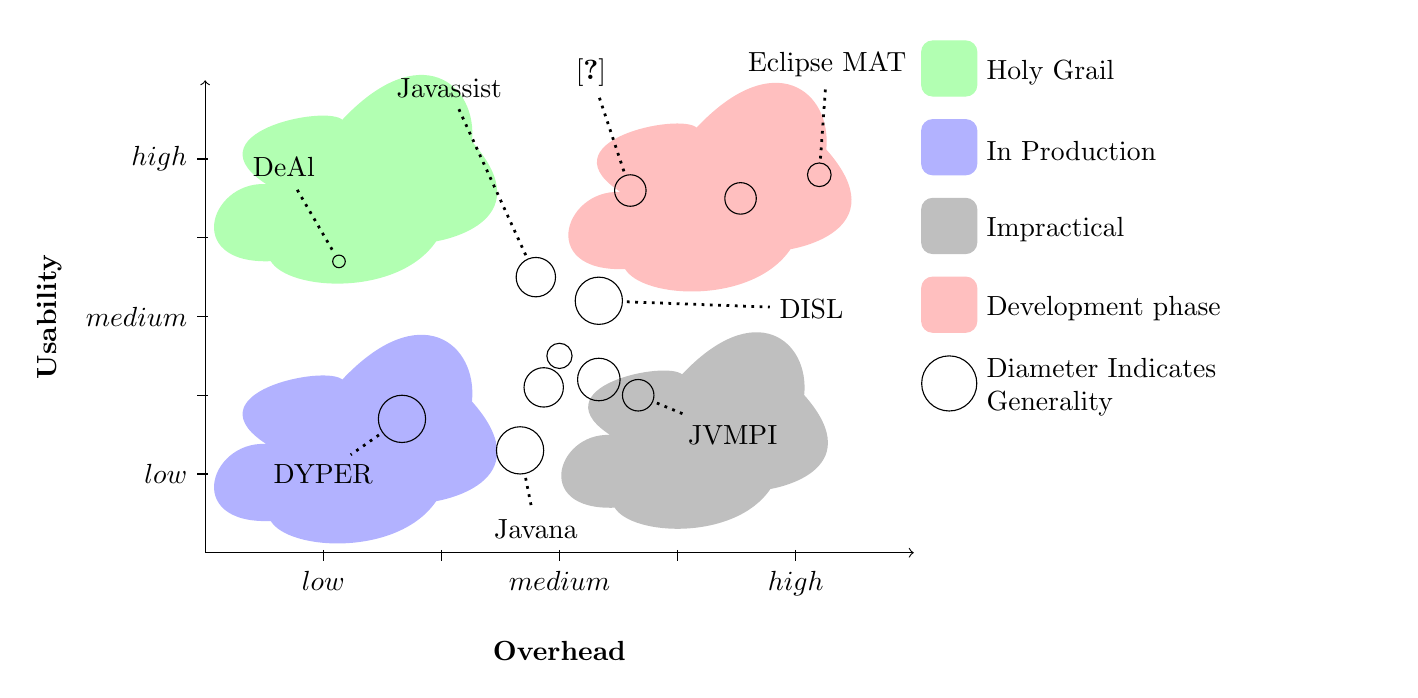
\begin{tikzpicture}
  \draw[->,xshift=0cm] (0,0) -- coordinate (x axis mid) (9,0);
  \draw[->,xshift=0cm] (0,0) -- coordinate (y axis mid) (0,6);
  \foreach \x/\xtext in {1.5/low,3/,4.5/medium,6/,7.5/high}
          \draw [xshift=0cm](\x cm,1pt) -- (\x cm,-3pt)
              node[anchor=north] {$\xtext$};
  \foreach \y/\ytext in {1/low,2/,3/medium,4/,5/high}
          \draw (1pt,\y cm) -- (-3pt,\y cm) node[anchor=east] {$\ytext$}; 
          
  \node[below=1cm] at (x axis mid) {\textbf{Overhead}};
  \node[rotate=90, above=1.7cm] at (y axis mid) {\textbf{Usability}};  
  % good region
  \node (cloudgood) at (2,4.9) {\tikz \asymcloud[0.17]{fill=green!30, draw=green!30,thick};};

  %\filldraw[fill=green, draw=green, rounded corners] (0.5,5.5) rectangle (3.5,3);
  
  %bad region
  \node (cloudbad) at (6.3,1.7) {\tikz \asymcloud[0.16]{fill=gray!50, draw=gray!50,thick};};
  
  %useful during development region
  \node (clouddevelopment) at (6.5,4.8) {\tikz \asymcloud[0.17]{fill=pink, draw=pink,thick};};

  %useful in production but not easy to use's region
  \node (cloudproduction) at (2,1.6) {\tikz \asymcloud[0.17]{fill=blue!30, draw=blue!30,thick};};

  % legend
  \filldraw[fill=green!30, draw=green!30, rounded corners] (9.1,6.5) rectangle (9.8,5.8);
  \node[right=0.7cm] at (9.1,6.1) {Holy Grail};
  
  \filldraw[fill=blue!30, draw=blue!30, rounded corners] (9.1,5.5) rectangle (9.8,4.8); 
  \node[right=0.7cm] at (9.1,5.1) {In Production};
  
  \filldraw[fill=gray!50, draw=gray!50, rounded corners] (9.1,4.5) rectangle (9.8,3.8);
  \node[right=0.7cm] at (9.1,4.1) {Impractical};
  
  \filldraw[fill=pink, draw=pink, rounded corners] (9.1,3.5) rectangle (9.8,2.8);
  \node[right=0.7cm] at (9.1,3.1) {Development phase};
  
  \draw (9.45,2.15) circle [radius=0.35];
  \node[right=0.7cm, text width = 5cm, align=left] at (9.1,2.1) {Diameter Indicates\\ Generality};
  
  % very general radius = 0.3
  % general radius = 0.2
  % limited radius = 0.1
  
   
  
  % JVMPI - medium usability - high overhead - average generality
  \draw[draw=black] (5.5,2) circle [radius=0.2cm];
  \path (5.5,2) node[circle,minimum size=0.5cm](JVMPI) {}
  		(6.7,1.5) node(JVMPIT) {JVMPI};
  \draw[draw=black,dotted, line width = 1pt] (JVMPI) -- (JVMPIT);
  %\node at (0.5,5.5) {\cite{Liang1999}};
  
  % JAVANA - low usability - medium overhead - high generalidad
  \draw[draw=black] (4,1.3) circle [radius=0.3cm];
  \path (4,1.3) node[circle,minimum size=0.7cm](JAVANA) {}
    		(4.2,0.3) node(JAVANAT) {Javana};
  \draw[draw=black,dotted, line width = 1pt] (JAVANA) -- (JAVANAT);
  
  % Binder CPU Profiling - medium overhead - medium/low usabilityc - low/medium generalidad 
  \draw[draw=black] (4.5,2.5) circle [radius=0.16cm]; % no
  
  % DYPER - medium/low overhead - low usability - high generalidad
  \draw[draw=black] (2.5, 1.7) circle [radius=0.3cm];
  \path (2.5, 1.7) node[circle,minimum size=0.7cm](DYPER) {}
      		(1.5,1) node(DYPERT) {DYPER};
  \draw[draw=black,dotted, line width = 1pt] (DYPER) -- (DYPERT);
  
  % ASM - medium overhead - low/medium usability - high generalidad
  \draw[draw=black] (4.3,2.1) circle [radius=0.25cm]; % [above=0.1]-- (2.3,2.7) node {ASM};
  
  % Javaassist - medium overhead - medium/high usability - high generality
  \draw[draw=black] (4.2,3.5) circle [radius=0.25cm];
  \path (4.2,3.5) node[circle,minimum size=0.6cm](Javassist) {}
        		(3.1,5.9) node(JavassistT) {Javassist};
  \draw[draw=black,dotted, line width = 1pt] (Javassist) -- (JavassistT);
  
  % Profiling with AspectJ - high usability - high overhead - averagage generality
  \draw[draw=black] (6.8,4.5) circle [radius=0.2cm]; % [above=0.1]-- (6.3,5) node {\cite{Pearce:2007:PA:1248445.1248448}};
  
  % Binder Major/AspectJ - medium overhead - high usability - average generalidad
  \draw[draw=black] (5.4,4.6) circle [radius=0.2cm];
  \path (5.4,4.6) node[circle,minimum size=0.5cm](Major) {}
          		(4.9,6.1) node(MajorT) {\cite{Binder:2006:FEM:1173706.1173733}};
  \draw[draw=black,dotted, line width = 1pt] (Major) -- (MajorT);
  
  % DISL - medium overhead - medium usability - full generalidad
  \draw[draw=black] (5,3.2) circle [radius=0.3cm];
  \path (5,3.2) node[circle,minimum size=0.7cm](DISL) {}
        (7.7,3.1) node(DISLT) {DISL};
  \draw[draw=black,dotted, line width = 1pt] (DISL) -- (DISLT);
  
  % Customized aspect weavers - medium overhead - low usability - full generalidad
  \draw[draw=black] (5, 2.2) circle [radius=0.27cm];
  
  % Eclipse MAT/ Visual VM/ YourKit - high overhead - meidum/high usability - limited/medium
  \draw[draw=black] (7.8,4.8) circle [radius=0.15cm];
  \path (7.8,4.8) node[circle,minimum size=0.4cm](Eclipse) {}
        (7.9,6.2) node(EclipseT) {Eclipse MAT};
  \draw[draw=black, dotted, line width = 1pt] (Eclipse) -- (EclipseT);
  
  % DeAl - low overhead - medium/high usability - limited generalidad
  \draw[draw=black] (1.7,3.7) circle [radius=0.08cm];
  \path (1.7,3.7) node[circle,minimum size=0.17cm](DeAl) {}
        (1,4.9) node(DeAlT) {DeAl};
  \draw[draw=black, dotted, line width = 1pt] (DeAl) -- (DeAlT);
  
\end{tikzpicture}
\caption{Assessing the relevance of the aforementioned approaches. The location in terms of overhead a usability is given for each approach. Furthermore, the area of each circumference indicates how general the approach is (the larger the better).} \label{fig:position-approaches-to-simplify}
\end{figure}

\section{Summary}


Defining and using software abstractions is at the core of systems development.
Once a new abstraction is defined, the tools used in the development process and to support resource awareness should be modified to make them reflect the new concepts.
When these modifications are not done, we argue that a mismatch exists between developer's view and the tooling's view.
Alas, implementing this tooling support is tedious and error-prone.
In this chapter, we have identified two challenges related to this complexity:

\begin{itemize}
\item A concrete abstraction may have specific features to consider when implementing tooling support.
By adding new requirements to the tools, these features hinder their implementation.
At the same time, some features can be useful to drive the behavior of systems that require support for resource awareness.

\item Since new software abstractions are defined all the time (for example, using DSLs), it is necessary to ease the task of building their tooling support.
For instance, building a resource consumption monitor for a new DSL should be simple enough as to make it affordable for DSL developers.
\end{itemize}   

In reviewing the state of the art of resource management for software abstractions, we realized that severe shortcomings in existing approaches prevent their usage in production environments.
With regard to the matter of dealing with abstraction-specific features, the following issues exist:

\begin{itemize}
\item Existing solutions offer limited support for resource accounting in component-based systems.
Besides targeting only mainstream component models; they induce, in general, high performance overhead. 

\item Most approaches that target component-based systems use little information about the architecture of the systems.
In those cases where such knowledge is used, the goal is solely to improve the accuracy of resource consumption monitoring.

\item Mechanisms exist to ease the construction of debuggers for new DSLs.
As far as we know, no similar mechanism for profilers have been proposed.

\end{itemize}

In addition, it is our opinion that current approaches, to build tooling support, lack the required simplicity and maturity. In particular:

\begin{itemize}
\item A deep understanding of low-level details of the target MRTE is often required to build tools for resource awareness.

\item Memory profilers offer extension capabilities.
Unfortunately, such extensions suffer from high overhead because they depend on methods to collect data that offer poor performance.

\item Although several approaches are able to produce complex dynamic analysis tools, most of them are not capable of delivering such functionality with low overhead.
Interestingly, the mechanisms that do offer a low overhead either require extensive knowledge of the platform or are limited in the kind of analysis they can perform.
\end{itemize} 


